
\subsection{Slow Controls}

\subsubsection{Framework}
\label{sec:ctrls:framework}
As any complex high energy and nuclear physics experiment HPS needs a sophisticated experimental controls 
system which will incorporate the existing slow controls components in Hall B, as well as 
newly developed subsystems.  The slow controls for HPS  will be based on the 
Experimental Physics and Industrial Control System (EPICS) framework. This choice is primarily 
driven by the necessity to be compatible with the existing Hall B and CEBAF slow controls systems. 
It will allow us to control  hardware used in the experiment from the counting house 
over the Ethernet, and we will benefit from numerous existing software components developed by the EPICS 
community, such as alarm systems, archivers, and setpoint save-and-restore software. EPICS Input/Output 
Controllers (IOC's)  will run on the rack-mountable 
Linux servers in the rack-room of the Hall B counting house and on the VME controllers in the Hall 
running either VxWorks or Linux operating systems. These IOC's will serve EPICS process variables 
to multiple clients over Ethernet using ChannelAccess (CA) protocol. The operators in the counting house 
will be able to monitor and change the parameters of the controlled hardware whenever necessary using 
CA-clients that have direct access to the slow controls network of Hall B.  
For control and alarm screens HPS will use Controls System Studio (CSS) framework which will also be  
used by the CLAS12 slow controls group. CSS provides a modern Java-based display management tool called 
BOY that allows the developer to quickly crate very dynamic control screens. We also currently plan to use 
the alarm framework developed by the controls group of Spallation Neutron Source at ORNL and is already integrated 
with CSS. The HPS experiment control system includes multiple components such as control and monitoring of  SVT, 
ECal, and the muon system's power supplies, beamline components and temperature monitoring. Each of 
these subsystems needs to have an EPICS interface to be controlled remotely from the counting house during 
the running. The subsections below briefly describe the main HPS slow control components. 


\subsubsection{Voltage controls}
\label{sec:ctrls:voltage}
Operation of the HPS silicon detectors requires bias voltages and three different types of low voltages: DVDD, 
AVDD and V125 (see Sec.~\ref{sec:svt} and Ref.~\cite{HPS_PROP}). Bias voltages will be adjustable up to 
500~\textmd{V}, while the other three will be fixed  at preset values. All four types of power  
will be provided by two different models of Wiener MPOD based boards: the MPV8008 8-channel low voltage boards and 
the EHS F205-F 16 channel high voltage boards. Because HPS silicon detectors use 36 hybrids and each hybrid requires 
three low voltage channels and one high voltage channel, we will need total of 14 MPV8008 boards and four EHS F205-F boards. 
The MPV8008 boards allow for voltage regulation at the desired sensor locations to account for the voltage drop due to the 
current draw in the low voltage circuits. Bias voltages can only be regulated only at the terminals, 
but their current draws are negligible. Wiener MPOD chassis can be remotely controlled and monitored over Ethernet using 
standard SNMP protocol. EPICS support for these boards and chassis already exists and has been successfully used at Jefferson Lab. 
It allows for automatic generation of the list of EPICS variables  by reading out the content of the MPOD chassis 
during IOC initialization stage. An EPICS application running on a rack-mountable Linux server will  
continuously monitor and modify the parameters of the boards using SNMP protocol.  
The set-points and readback values of the parameters will be archived using EPICS archiver developed and maintained 
by the the controls group of Jefferson Lab Accelerator division. 
HPS-specific control and alarm screens will be developed similar to those used during 2012 HPS test run in 
Hall B, see Figure~\ref{fig:svt_power}. 
  
\begin{figure*}[t]
\begin{center}
%\epsfig{file=slow_control/svt_voltage_gui.eps,width=\textwidth,angle=0}
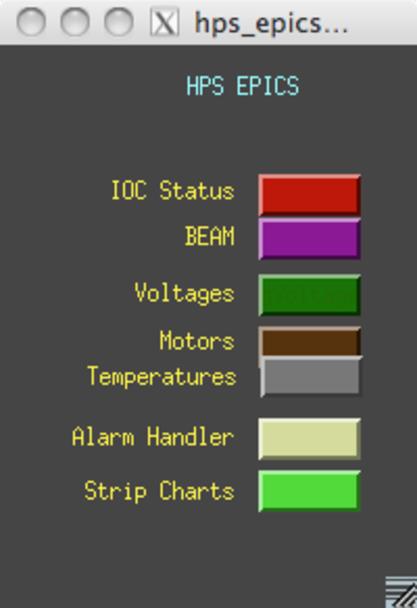
\includegraphics[width=0.15\textwidth]{slow_control/hps_epics}
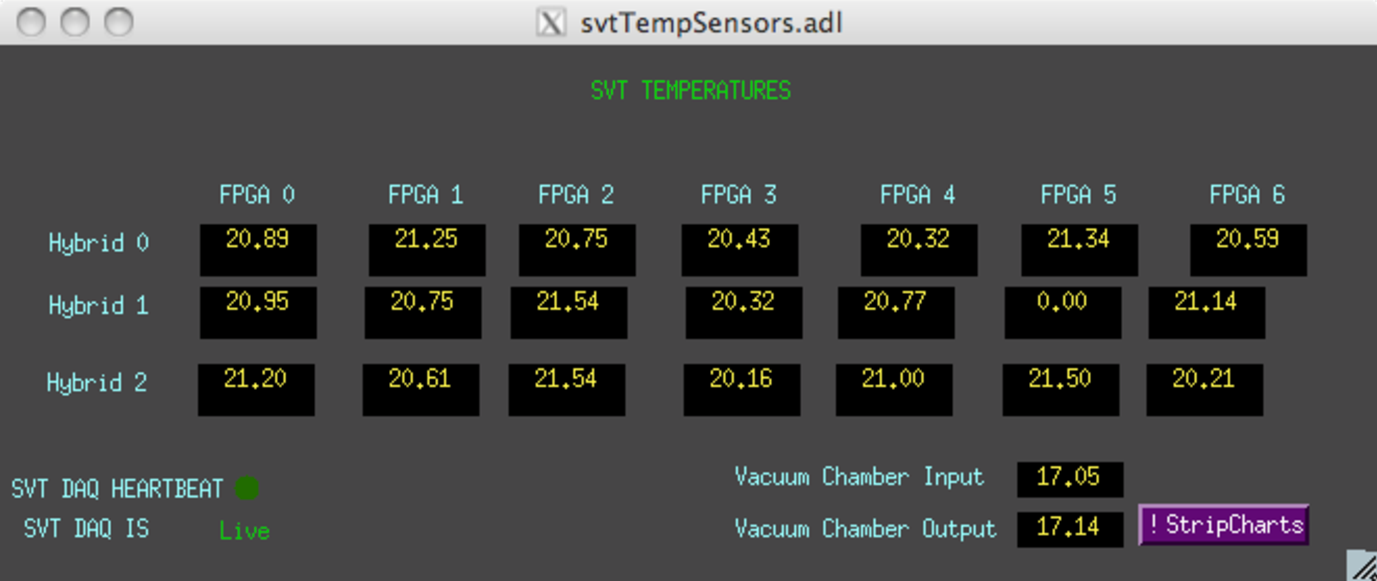
\includegraphics[width=0.55\textwidth]{slow_control/SVT_temp_monitor}
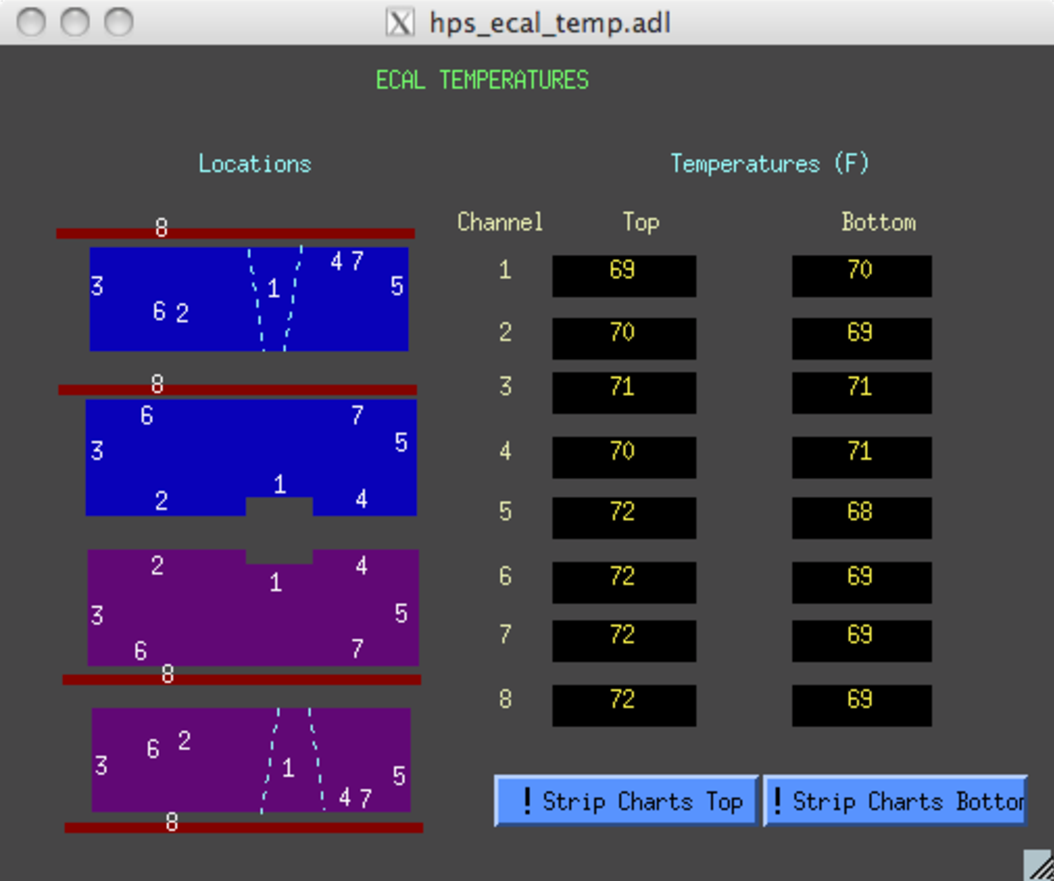
\includegraphics[width=0.275\textwidth]{slow_control/ECal_temp_monitor}
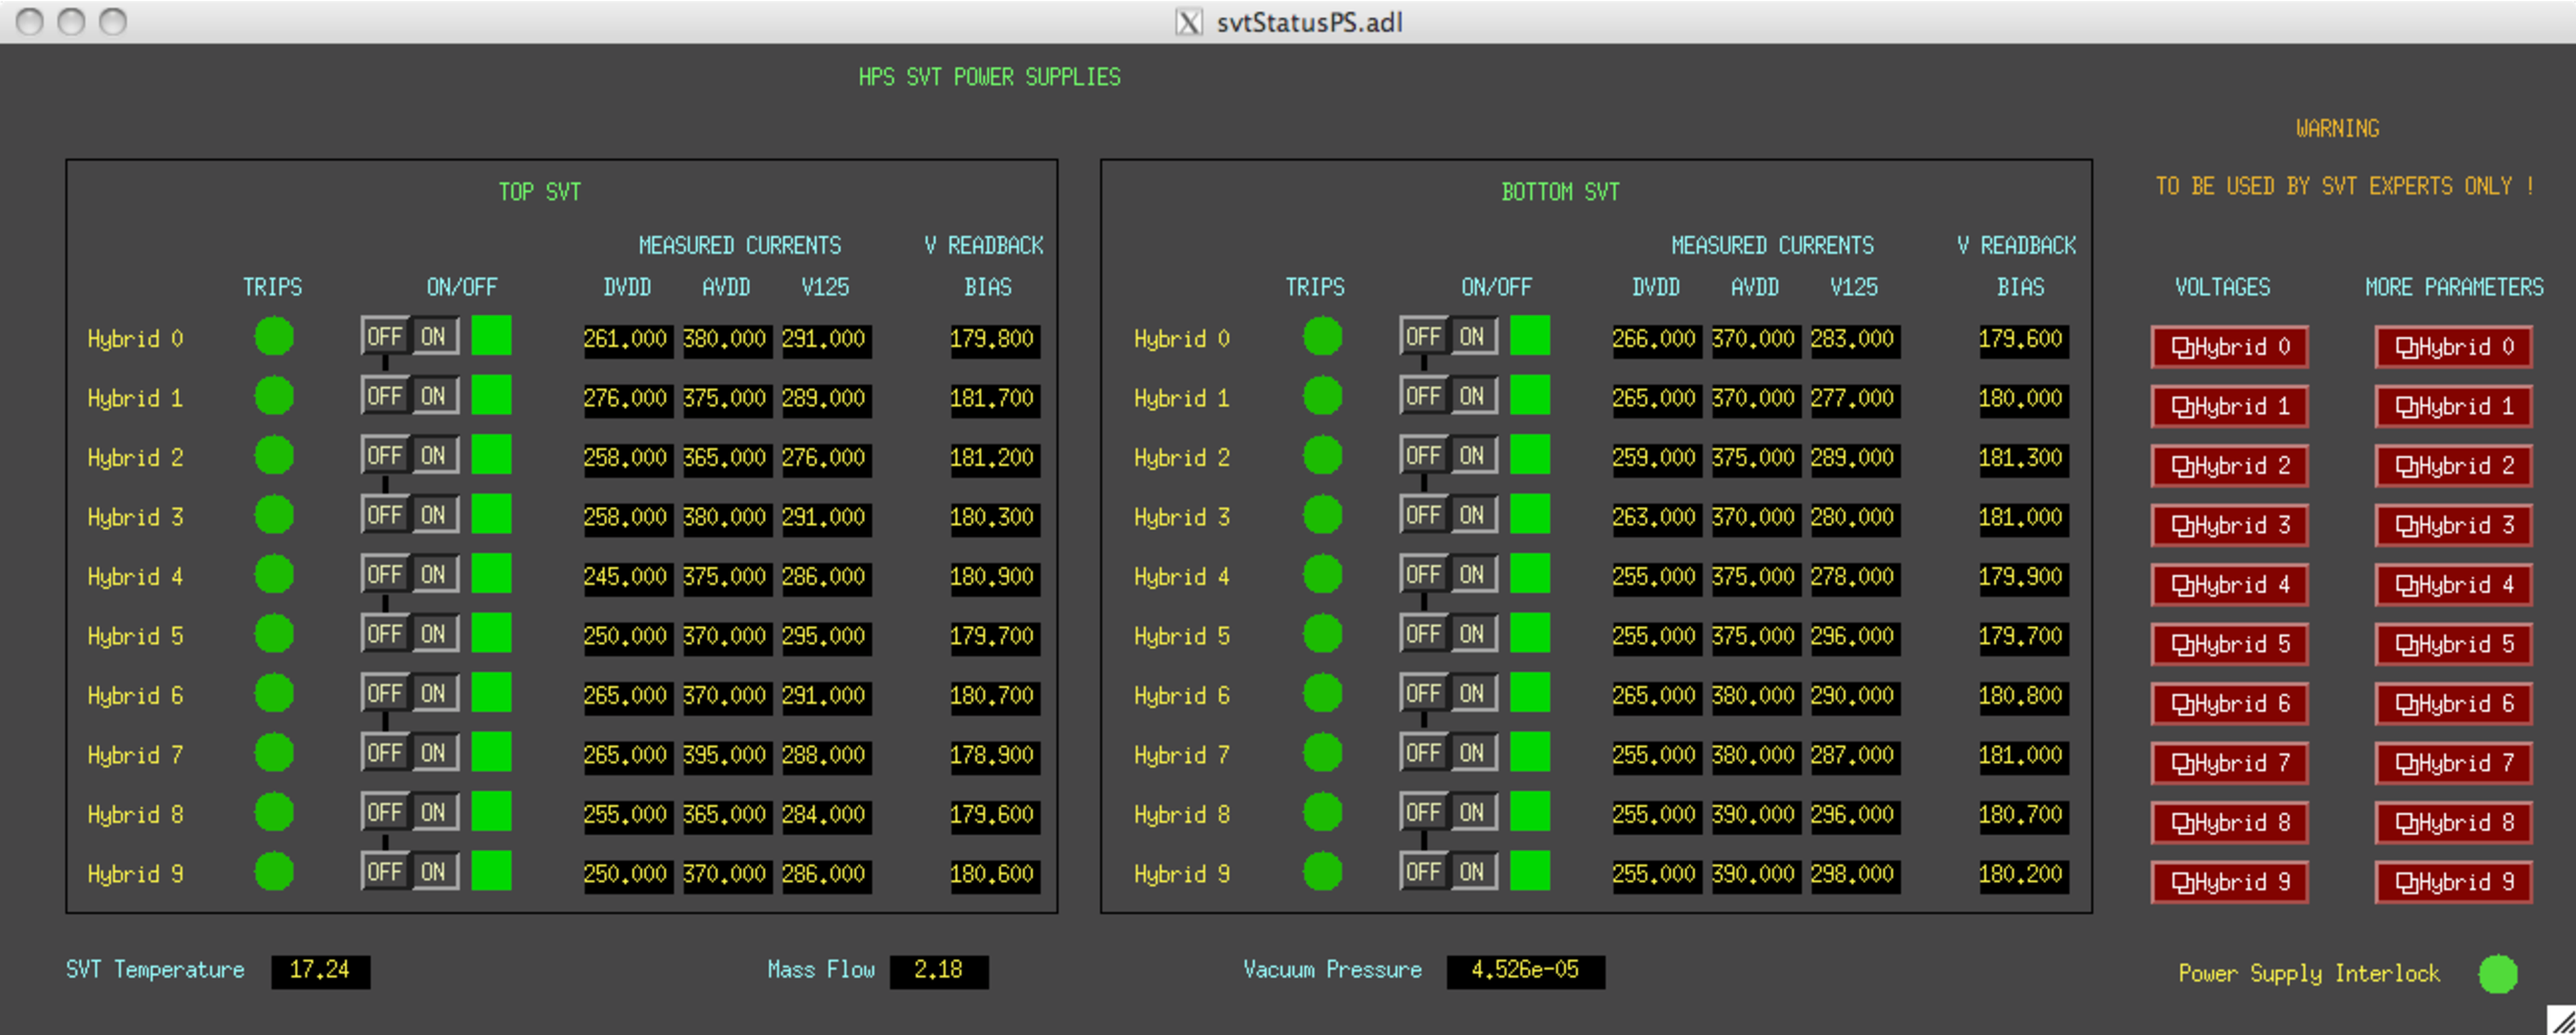
\includegraphics[width=\textwidth]{slow_control/SVT_HV_control_monitor}
\caption{Voltage and temperature control screens during 2012 test run in Hall B. Similar control screens will be developed for 
2014 run using CSS BOY display management framework.}
\label{fig:svt_power}
\end{center}
%\label{fig:ctrls_svt_power}
\end{figure*}

The power for APD's of the ECal and for the PMTs of the muon system  will be provided by the   
CAEN SY1527 high voltage chassis. CAEN A1520 boards will power the ECal APDs while CAEN A1535 boards will 
provide high voltage to the PMTs of the muon system. CAEN SY1527 chassis can be remotely controlled over Ethernet 
using a proprietary protocol. EPICS interface for the SY1527 chassis already exists and it has been successfully 
used at Jefferson Lab and other laboratories world-wide. The EPICS IOC for the ECal and muon voltage 
control will run on a rack-mountable computer in the counting house and serve the voltage-related process 
variables to other ChannelAccess clients. High voltage control screens will be designed 
similar to those used for CLAS IC and EC voltage control GUIs. The alarm system will be configured to alert 
the shift personnel and annunciate deviation of the HV channels readback from its demand voltage values as  
well as of the trip state of the channels set by the chassis itself.    


\subsubsection{Motor controls}
\label{sec:ctrls:motor}
The HPS experiment will use eight applications requiring motion control. Three of them 
are the standard Hall B PMT-based beamline harps at 2C21, 2C24 and 2H00 locations,  and the controls 
and analysis software for them will not change.  HPS will use the ``long radiator'' ladder of CLAS to align  
the SVT collimator with the electron beamline as described in Sec.~\ref{setup:beamline}, and only minor 
modifications to the existing software will be required to control the position of the collimator.
Another Hall B piece of equipment that was used by a number of experiments is the beam blocker that is inserted 
into the beam line to protect the Faraday cup in the electron beam dump from excessive beam currents. The 
controls hardware and software for the beam blocker will be identical to that used by CLAS. 

HPS will require development of three additional stepper motor-based applications. 
First, as it was discussed in Sec.~\ref{setup:beam_dignostics}, the two mounting frames of the silicon detectors 
will hold four wires for SVT alignment with respect to the electron beam. Second, the two thin 
tungsten targets used in HPS will be changeable depending on the beam and run conditions. The target 
positions will be controlled by a single stepper motor, while the positions of the upper and lower 
modules will be independently controlled by two separate stepper motors. 

All motors used by HPS  will be powered by Oregon Micro Systems (OMS) PMD4 drivers housed in custom-designed chassis 
that contain four PMD4 boards. The chassis provide connections for the power, limit and home switches and, the encoder. 
The computer interface is provided by OMS VS4 VME boards, each capable of controlling four motion axes.  
This is the standard configuration that was  used for all of the motor-based applications in Hall B. Therefore, 
HPS does not need to develop software for basic motor control with EPICS, and will simply take advantage of the existing 
framework used by CLAS.

Higher tier controls and online analysis software required for the SVT wire scans will be developed on the basis of 
the existing software for the Hall B harp scans.  
The relative position of the silicon detectors with respect to the beamline will be determined by slowly moving 
a wire in the transverse direction across the beam and by measuring at different wire positions the scaler rates from 
the beam halo counters mounted around the beam-pipe downstream of the silicon detectors. The speed of the wire, the motion 
range, and the sampling rate will be tuned during the commissioning of the experiment. The scan software will perform 
an online analysis of the acquired data and the resulting plots from each scan will look similar to the plots presented in 
Fig.~\ref{fig:profile_test}. Using the locations of the peaks in the counting rates determined by a fit to a Gaussian 
distribution, one should be able to optimize the alignment of silicon detectors with respect to the electron beam.



\subsubsection{Magnet controls}
\label{sec:ctrls:magnet}
During the HPS run in 2014 we plan to use existing magnets that were used in previous Hall B experiments: 
the tagger magnet to bend the electrons into the tagger dump during beam tuning; Hall B pair spectrometer dipole magnet 
as the analyzing magnet, and two H-type chicane magnets. As described in Section~\ref{setup:layout}, all four magnets have 
fully operational power supplies with controls hardware and software already installed. Therefore, no additional 
effort will be required to be able to control the HPS magnets.     
   


\subsubsection{Temperature control and monitoring}
\label{sec:ctrl:temp}
Both ECal and SVT readout electronics will need temperature stabilization, therefore both components  
will have cooling systems requiring two separate chillers. ECal will utilize the 
existing chiller that was used for CLAS Inner Calorimeter and that does not need an external 
control. For the SVT cooling system HPS will purchase a new chiller which will allow for a remote control 
and monitoring through a serial connection. HPS slow controls group will develop EPICS support for the new SVT 
chiller to be able to monitor its status and change the temperature setpoint remotely during the experiment.   

The temperature monitoring of ECal will use thermocouples mounted on the ECal electronics. HPS slow controls group will 
develop EPICS readout software for these thermocouples based on the prototype system 
used during the 2012 HPS beam test. The SVT temperature monitoring will be done using the internal temperature 
sensors read out by the SVT data acquisition system. An EPICS IOC will serve records to hold the SVT temperature 
values while a client on the SVT DAQ will regularly update the values of these records. In addition, 
the temperature at the entrance and the exit of the vacuum chamber will also be measured  
using thermocouples similar to those used for ECal which will allow us to continuously monitor the SVT ambient 
temperature independent of the SVT DAQ status.  

In order to safely operate silicon detectors a number of interlocks will need to be set similar to those 
used during 2012 HPS beam test.  Because the silicon detectors will operate in vacuum it is crucial 
to maintain  coolant flow through the system when the silicon detectors are powered. The flow of the 
coolant has to be turned off in the event of deteriorating vacuum, as a precaution to prevent any potential fluid 
leakage into the vacuum chamber. If the readings for the temperature or pressure in the vacuum chamber exceeds its
respective threshold value, the power to the SVT and the flow in the SVT cooling system
will be shut off using a hardware interlock system. The mass flow of the coolant, the vacuum 
pressure, and the status of the interlock components will be continuously readout and monitored via EPICS.

